\section{Introduction}
The Backlog and Traceability document presents all the identified requirements related to the project. It describes how we have implemented Scrum and how Scrum deals with requirements. Next it presents how we ensure traceability and an overview over all the requirements and their status. Lastly it includes a list of activities or tasks we have done in various Sprints throughout our project. \\
\\
The requirements in Scrum are represented by "User Stories". These stories are short descriptive text written with the end-user in mind. Instead of using a traditional ranking system, Scrum says that, whatever is on top of the Product Backlog is the most important. In our case this means that we can keep a "red line" in the Backlog where all items over this line is "must do's", and those below are "can do's". 
We are using Jira Project Managment tool to facilitate our project and to keep track of all needs and user stories. Jira provides us with some useful features such as Sprint Health (Fig. \ref{fig:sh}) and Burndown charts(Fig. \ref{fig:bdc}). All our activities gets a uniqe Jira ID named \textbf{VPQ-000} which is automatically generated by Jira \\
\\ 

\begin{figure}[h]
        \centering
         \begin{minipage}[b]{0.3\textwidth}
            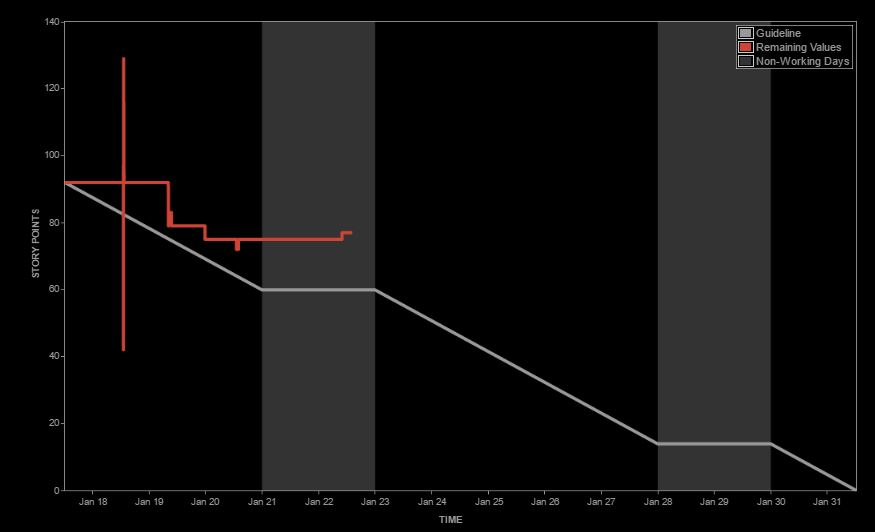
\includegraphics[width = 1\textwidth]{VAPIQ-PICTURES/BDC}
            \caption{Burndown Chart}
            \label{fig:bdc}
        \end{minipage}
        \hfill
        \begin{minipage}[b]{0.6\textwidth}
            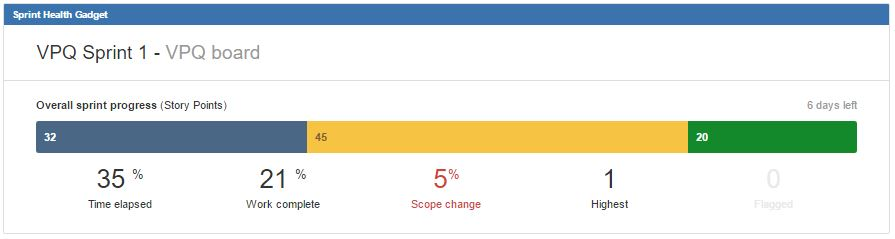
\includegraphics[width = 1\textwidth]{VAPIQ-PICTURES/SH}
            \caption{Sprint Health}
            \label{fig:sh}
        \end{minipage}
\end{figure}


\vspace*{1cm}
\noindent
We are dependent on an external tracking system, located at KONGSBERG Innovation Center (KIC), named Qualisys. This is a motion tracking system which uses small reflective bullets to track the motion and position of the object they are placed on. By using this system, we should be able to create reproducible test results. We are going to write our own flight controller using real-time data received from Qualisys. 
\\ 

